

\tikzset{every picture/.style={line width=0.75pt}} %set default line width to 0.75pt

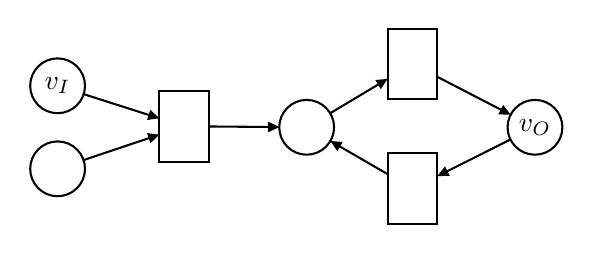
\begin{tikzpicture}[x=0.75pt,y=0.75pt,yscale=-1,xscale=1]
%uncomment if require: \path (0,128); %set diagram left start at 0, and has height of 128


% Text Node
\draw  [fill={rgb, 255:red, 255; green, 255; blue, 255 }  ,fill opacity=1 ]  (29, 41) circle [x radius= 13.2, y radius= 13.2]   ;
\draw (29,41) node   [align=left] {\begin{minipage}[lt]{14.96pt}\setlength\topsep{0pt}
\begin{center}
$\displaystyle v_{I}$
\end{center}

\end{minipage}};
% Text Node
\draw  [fill={rgb, 255:red, 255; green, 255; blue, 255 }  ,fill opacity=1 ]  (29, 81) circle [x radius= 13.2, y radius= 13.2]   ;
\draw (29,81) node   [align=left] {\begin{minipage}[lt]{14.96pt}\setlength\topsep{0pt}
\begin{center}
\end{center}

\end{minipage}};
% Text Node
\draw  [fill={rgb, 255:red, 255; green, 255; blue, 255 }  ,fill opacity=1 ]  (78,43.5) -- (102,43.5) -- (102,77.5) -- (78,77.5) -- cycle  ;
\draw (90,60.5) node   [align=left] {\begin{minipage}[lt]{13.600000000000001pt}\setlength\topsep{0pt}
\begin{center}
\end{center}

\end{minipage}};
% Text Node
\draw  [fill={rgb, 255:red, 255; green, 255; blue, 255 }  ,fill opacity=1 ]  (149, 61) circle [x radius= 13.2, y radius= 13.2]   ;
\draw (149,61) node   [align=left] {\begin{minipage}[lt]{14.96pt}\setlength\topsep{0pt}
\begin{center}
\end{center}

\end{minipage}};
% Text Node
\draw  [fill={rgb, 255:red, 255; green, 255; blue, 255 }  ,fill opacity=1 ]  (188,13.5) -- (212,13.5) -- (212,47.5) -- (188,47.5) -- cycle  ;
\draw (200,30.5) node   [align=left] {\begin{minipage}[lt]{13.600000000000001pt}\setlength\topsep{0pt}
\begin{center}
\end{center}

\end{minipage}};
% Text Node
\draw  [fill={rgb, 255:red, 255; green, 255; blue, 255 }  ,fill opacity=1 ]  (188,73.5) -- (212,73.5) -- (212,107.5) -- (188,107.5) -- cycle  ;
\draw (200,90.5) node   [align=left] {\begin{minipage}[lt]{13.600000000000001pt}\setlength\topsep{0pt}
\begin{center}
\end{center}

\end{minipage}};
% Text Node
\draw  [fill={rgb, 255:red, 255; green, 255; blue, 255 }  ,fill opacity=1 ]  (259, 61) circle [x radius= 13.2, y radius= 13.2]   ;
\draw (259,61) node   [align=left] {\begin{minipage}[lt]{14.96pt}\setlength\topsep{0pt}
\begin{center}
$\displaystyle v_{O}$
\end{center}

\end{minipage}};
% Connection
\draw    (41.58,45.02) -- (75.14,55.75) ;
\draw [shift={(78,56.66)}, rotate = 197.73] [fill={rgb, 255:red, 0; green, 0; blue, 0 }  ][line width=0.08]  [draw opacity=0] (5.36,-2.57) -- (0,0) -- (5.36,2.57) -- cycle    ;
% Connection
\draw    (41.52,76.79) -- (75.16,65.49) ;
\draw [shift={(78,64.53)}, rotate = 521.4200000000001] [fill={rgb, 255:red, 0; green, 0; blue, 0 }  ][line width=0.08]  [draw opacity=0] (5.36,-2.57) -- (0,0) -- (5.36,2.57) -- cycle    ;
% Connection
\draw    (102,60.6) -- (132.8,60.86) ;
\draw [shift={(135.8,60.89)}, rotate = 180.49] [fill={rgb, 255:red, 0; green, 0; blue, 0 }  ][line width=0.08]  [draw opacity=0] (5.36,-2.57) -- (0,0) -- (5.36,2.57) -- cycle    ;
% Connection
\draw    (160.33,54.22) -- (185.43,39.22) ;
\draw [shift={(188,37.68)}, rotate = 509.12] [fill={rgb, 255:red, 0; green, 0; blue, 0 }  ][line width=0.08]  [draw opacity=0] (5.36,-2.57) -- (0,0) -- (5.36,2.57) -- cycle    ;
% Connection
\draw    (212,36.7) -- (244.61,53.56) ;
\draw [shift={(247.27,54.94)}, rotate = 207.34] [fill={rgb, 255:red, 0; green, 0; blue, 0 }  ][line width=0.08]  [draw opacity=0] (5.36,-2.57) -- (0,0) -- (5.36,2.57) -- cycle    ;
% Connection
\draw    (247.19,66.9) -- (214.68,83.16) ;
\draw [shift={(212,84.5)}, rotate = 333.43] [fill={rgb, 255:red, 0; green, 0; blue, 0 }  ][line width=0.08]  [draw opacity=0] (5.36,-2.57) -- (0,0) -- (5.36,2.57) -- cycle    ;
% Connection
\draw    (188,83.56) -- (163.03,69.11) ;
\draw [shift={(160.43,67.61)}, rotate = 390.05] [fill={rgb, 255:red, 0; green, 0; blue, 0 }  ][line width=0.08]  [draw opacity=0] (5.36,-2.57) -- (0,0) -- (5.36,2.57) -- cycle    ;

\end{tikzpicture}